% Practice Test 04 — Florida Edition
% Questions: 30 (21 MC + 9 SA)
% Generated by scripts/generate_practice_tests.py

\begin{practiceQuestion}{1-3-q06}{mc}
\begin{questionText}
On a proportional graph, the point $(1, r)$ represents:
\end{questionText}
\choiceA{The $x$-intercept}
\choiceB{The constant of proportionality}
\choiceC{The slope of the line}
\choiceD{Both B and C}
\correctAnswer{D}
\explanation{At $x = 1$, $y = k \times 1 = k$. So the point $(1, r)$ gives the constant of proportionality, which is also the slope.}
\end{practiceQuestion}

\begin{practiceQuestion}{1-6-q06}{mc}
\begin{questionText}
Small paint can: $\frac{3}{4}$ gallon for $\$18$. Large can: $1\frac{1}{2}$ gallons for $\$33$. Which is the better buy?
\end{questionText}
\choiceA{Small, at $\$22$/gal}
\choiceB{Large, at $\$22$/gal}
\choiceC{Small, at $\$24$/gal}
\choiceD{Large, at $\$24$/gal}
\correctAnswer{B}
\explanation{Small: $18 \div 0.75 = \$24$/gal. Large: $33 \div 1.5 = \$22$/gal. The large can is $\$2$/gal cheaper.}
\end{practiceQuestion}

\begin{practiceQuestion}{2-1-q04}{mc}
\begin{questionText}
A class has $32$ students. If $75\%$ passed the test, how many students passed?
\end{questionText}
\choiceA{$20$}
\choiceB{$24$}
\choiceC{$25$}
\choiceD{$28$}
\correctAnswer{B}
\explanation{$75\% = 0.75$. Multiply: $0.75 \times 32 = 24$ students passed.}
\end{practiceQuestion}

\begin{practiceQuestion}{2-2-q11}{mc}
\begin{questionText}
A recipe uses $3$ cups of sugar out of $12$ cups of ingredients total. What percent is sugar?
\end{questionText}
\choiceA{$20\%$}
\choiceB{$25\%$}
\choiceC{$30\%$}
\choiceD{$36\%$}
\correctAnswer{B}
\explanation{$\frac{3}{12} = \frac{p}{100}$. Cross-multiply: $12p = 300$. Divide: $p = 25\%$.}
\end{practiceQuestion}

\begin{practiceQuestion}{2-6-q13}{mc}
\begin{questionText}
You want to earn $\$200$ in interest in $4$ years at $5\%$ simple interest. How much must you deposit?
\end{questionText}
\choiceA{$\$800$}
\choiceB{$\$1{,}000$}
\choiceC{$\$1{,}200$}
\choiceD{$\$2{,}000$}
\correctAnswer{B}
\explanation{$200 = P \times 0.05 \times 4$ → $200 = 0.20P$ → $P = \$1{,}000$.}
\end{practiceQuestion}

\begin{practiceQuestion}{2-7-q24}{sa}
\begin{questionText}
You guessed there were $300$ people at a concert. The actual attendance was $350$. Find the percent error (rounded to the nearest tenth).
\end{questionText}
\correctAnswer{$\approx 14.3\%$}
\explanation{$\frac{|300 - 350|}{350} \times 100 = \frac{50}{350} \times 100 \approx 14.3\%$.}
\end{practiceQuestion}

\begin{practiceQuestion}{3-2-q28}{gmc}
\begin{questionText}
Look at the table of deposits and withdrawals from a bank account.

\begin{center}
\begin{tabular}{|c|c|}
\hline
\textbf{Day} & \textbf{Transaction} \\
\hline
Monday & $+\$30$ \\
\hline
Tuesday & $-\$45$ \\
\hline
Wednesday & $+\$20$ \\
\hline
Thursday & $-\$15$ \\
\hline
\end{tabular}
\end{center}

If the account started at $\$0$, what is the balance after Thursday?
\end{questionText}
\choiceA{$\$110$}
\choiceB{$-\$10$}
\choiceC{$\$10$}
\choiceD{$-\$50$}
\correctAnswer{B}
\explanation{$0 + 30 + (-45) + 20 + (-15) = 30 + 20 - 45 - 15 = 50 - 60 = -10$. The balance is $-\$10$.}
\end{practiceQuestion}

\begin{practiceQuestion}{3-3-q25}{sa}
\begin{questionText}
An airplane is at $30{,}000$ feet. It descends $8{,}500$ feet. What is the new altitude?
\end{questionText}
\correctAnswer{$21{,}500$ feet}
\explanation{$30{,}000 - 8{,}500 = 21{,}500$ feet.}
\end{practiceQuestion}

\begin{practiceQuestion}{4-4-q02}{mc}
\begin{questionText}
Factor $6x + 12$.
\end{questionText}
\choiceA{$2(3x + 6)$}
\choiceB{$6(x + 2)$}
\choiceC{$3(2x + 4)$}
\choiceD{$6(x + 12)$}
\correctAnswer{B}
\explanation{GCF of $6x$ and $12$ is $6$. Factor: $6x \div 6 = x$ and $12 \div 6 = 2$. Result: $6(x + 2)$.}
\end{practiceQuestion}

\begin{practiceQuestion}{4-5-q27}{gmc}
\begin{questionText}
A pentagon has the side lengths shown below. What is the perimeter?

\begin{center}
\begin{tikzpicture}[scale=0.8]
  \coordinate (A) at (0,0);
  \coordinate (B) at (3,0);
  \coordinate (C) at (4,2);
  \coordinate (D) at (2,3.5);
  \coordinate (E) at (-1,2);
  \draw[thick, fill=funBlue!10] (A) -- (B) -- (C) -- (D) -- (E) -- cycle;
  \node[below] at (1.5,0) {$2x + 3$};
  \node[right] at (3.7,1) {$x + 1$};
  \node[above right] at (3.2,2.9) {$x - 2$};
  \node[above left] at (0.3,2.9) {$3x + 4$};
  \node[left] at (-0.7,1) {$x$};
\end{tikzpicture}
\end{center}
\end{questionText}
\choiceA{$8x + 6$}
\choiceB{$7x + 6$}
\choiceC{$8x + 8$}
\choiceD{$7x + 8$}
\correctAnswer{A}
\explanation{Add all sides: $(2x + 3) + (x + 1) + (x - 2) + (3x + 4) + x = (2x + x + x + 3x + x) + (3 + 1 - 2 + 4) = 8x + 6$.}
\end{practiceQuestion}

\begin{practiceQuestion}{5-3-q05}{mc}
\begin{questionText}
Solve $6(x - 1) = -18$.
\end{questionText}
\choiceA{$x = -2$}
\choiceB{$x = 2$}
\choiceC{$x = -4$}
\choiceD{$x = 4$}
\correctAnswer{A}
\explanation{Divide by $6$: $x - 1 = -3$. Add $1$: $x = -2$. Check: $6(-2 - 1) = 6(-3) = -18$ \checkmark.}
\end{practiceQuestion}

\begin{practiceQuestion}{5-4-q29}{gsa}
\begin{questionText}
The bar graph shows how much three students earned. Together they earned a total of $\$31.50$. Student C earned $\dfrac{1}{2}$ as much as Student A. Find how much Student C earned.

\begin{center}
\begin{tikzpicture}[scale=0.5]
  \draw[thick,->] (0,0) -- (0,11) node[above] {Dollars (\$)};
  \draw[thick,->] (0,0) -- (10,0);
  % Bars
  \draw[thick,fill=funBlue!40] (1,0) rectangle (3,8);
  \node[below] at (2,-0.3) {A};
  \node at (2,8.5) {$\$12$};
  \draw[thick,fill=funOrange!40] (4,0) rectangle (6,0);
  \node[below] at (5,-0.3) {B};
  \node at (5,1) {?};
  \draw[thick,fill=funGreen!40] (7,0) rectangle (9,0);
  \node[below] at (8,-0.3) {C};
  \node at (8,1) {?};
  % Y-axis labels
  \foreach \y in {0,2,...,10} {
    \draw (-0.2,\y) -- (0,\y);
    \node[left] at (-0.3,\y) {$\y$};
  }
\end{tikzpicture}
\end{center}

Student A earned $\$12$, and Student C earned $\dfrac{1}{2}$ of Student A's earnings.
\end{questionText}
\correctAnswer{$\$6$}
\explanation{Student C $= \frac{1}{2} \times 12 = \$6$. Check: Student B $= 31.50 - 12 - 6 = \$13.50$. Total: $12 + 13.50 + 6 = 31.50$ \checkmark.}
\end{practiceQuestion}

\begin{practiceQuestion}{5-5-q26}{gmc}
\begin{questionText}
Which inequality is represented by the number line below?

\begin{center}
\begin{tikzpicture}[scale=0.7]
  \draw[thick,->] (-1,0) -- (10,0);
  \foreach \x in {0,...,9} \draw (\x,0.15) -- (\x,-0.15) node[below] {$\x$};
  \draw[thick,funBlue,->] (5,0) -- (10,0);
  \draw[thick,funBlue,fill=white] (5,0) circle (4pt);
\end{tikzpicture}
\end{center}
\end{questionText}
\choiceA{$x \geq 5$}
\choiceB{$x > 5$}
\choiceC{$x \leq 5$}
\choiceD{$x < 5$}
\correctAnswer{B}
\explanation{An open circle at $5$ with shading to the right means $x > 5$ (not including $5$).}
\end{practiceQuestion}

\begin{practiceQuestion}{5-6-q13}{mc}
\begin{questionText}
True or false: The graph of $x < 5$ and $x \leq 5$ look exactly the same.
\end{questionText}
\choiceA{True — both shade to the left of $5$}
\choiceB{False — $x < 5$ has an open circle, $x \leq 5$ has a closed circle}
\choiceC{False — they shade in different directions}
\choiceD{True — the circle type does not matter}
\correctAnswer{B}
\explanation{$x < 5$ uses an open circle (not including $5$) while $x \leq 5$ uses a closed circle (including $5$). Both shade left.}
\end{practiceQuestion}

\begin{practiceQuestion}{6-2-q13}{mc}
\begin{questionText}
A drawing uses $1$ cm $= 6$ m. It is redrawn at $1$ cm $= 2$ m. The original drawing is $8$ cm by $5$ cm. What is the perimeter of the new drawing?
\end{questionText}
\choiceA{$26$ cm}
\choiceB{$39$ cm}
\choiceC{$78$ cm}
\choiceD{$120$ cm}
\correctAnswer{C}
\explanation{Scale ratio: $\frac{6}{2} = 3$. New dimensions: $8 \times 3 = 24$ cm and $5 \times 3 = 15$ cm. New perimeter: $2(24 + 15) = 78$ cm.}
\end{practiceQuestion}

\begin{practiceQuestion}{6-4-q15}{mc}
\begin{questionText}
You know two angles of a triangle are $55°$ and $65°$ and a non-included side is $9$ cm. This is an example of:
\end{questionText}
\choiceA{SSS}
\choiceB{SAS}
\choiceC{ASA}
\choiceD{AAS}
\correctAnswer{D}
\explanation{Two angles and a non-included side is AAS (Angle-Angle-Side). This produces a unique triangle.}
\end{practiceQuestion}

\begin{practiceQuestion}{6-5-q19}{sa}
\begin{questionText}
What shape is the cross-section when you cut a sphere through its center?
\end{questionText}
\correctAnswer{A circle (the largest possible circle)}
\explanation{A cut through the center of a sphere produces a great circle — the largest possible circular cross-section, with the same radius as the sphere.}
\end{practiceQuestion}

\begin{practiceQuestion}{6-6-q27}{gmc}
\begin{questionText}
In the diagram below, lines $AB$ and $CD$ intersect at point $O$. Find the value of $y$.

\begin{center}
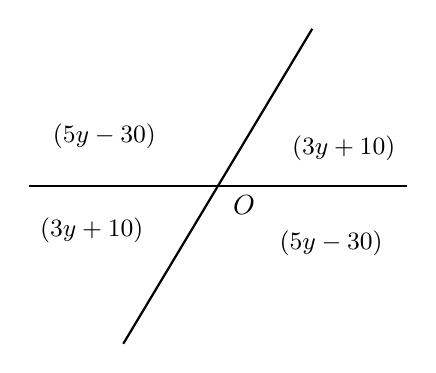
\begin{tikzpicture}[scale=0.8]
  \draw[thick] (-3,0) -- (3,0);
  \draw[thick] (-1.5,-2.5) -- (1.5,2.5);
  \node at (0,0) [below right,xshift=2pt] {$O$};
  \node at (2,0.6) {\small $(3y + 10)°$};
  \node at (-2,-0.7) {\small $(3y + 10)°$};
  \node at (-1.8,0.8) {\small $(5y - 30)°$};
  \node at (1.8,-0.9) {\small $(5y - 30)°$};
\end{tikzpicture}
\end{center}
\end{questionText}
\choiceA{$10$}
\choiceB{$20$}
\choiceC{$25$}
\choiceD{$35$}
\correctAnswer{C}
\explanation{Adjacent angles are supplementary: $(3y + 10) + (5y - 30) = 180$. Combine: $8y - 20 = 180$. Solve: $8y = 200$, $y = 25$.}
\end{practiceQuestion}

\begin{practiceQuestion}{7-1-q24}{sa}
\begin{questionText}
Two circles have radii of $4$ cm and $9$ cm. What is the difference between their diameters?
\end{questionText}
\correctAnswer{$10$ cm}
\explanation{Diameters: $2 \times 4 = 8$ cm and $2 \times 9 = 18$ cm. Difference: $18 - 8 = 10$ cm.}
\end{practiceQuestion}

\begin{practiceQuestion}{7-5-q01}{mc}
\begin{questionText}
What is the surface area of a cube with side length $4$ cm?
\end{questionText}
\choiceA{$16$ cm$^2$}
\choiceB{$64$ cm$^2$}
\choiceC{$96$ cm$^2$}
\choiceD{$24$ cm$^2$}
\correctAnswer{C}
\explanation{A cube has $6$ faces. $SA = 6s^2 = 6 \times 16 = 96$ cm$^2$.}
\end{practiceQuestion}

\begin{practiceQuestion}{7-6-q02}{mc}
\begin{questionText}
Which formula is used to find the volume of any prism?
\end{questionText}
\choiceA{$V = lwh$ only}
\choiceB{$V = Bh$}
\choiceC{$V = 2(lw + lh + wh)$}
\choiceD{$V = \frac{1}{3}Bh$}
\correctAnswer{B}
\explanation{The general formula for the volume of any prism is $V = Bh$, where $B$ is the area of the base and $h$ is the height.}
\end{practiceQuestion}

\begin{practiceQuestion}{7-7-q15}{mc}
\begin{questionText}
Which has more volume: a cylinder with $r = 3$ cm and $h = 10$ cm, or a cylinder with $r = 5$ cm and $h = 3$ cm? Use $\pi \approx 3.14$.
\end{questionText}
\choiceA{The first cylinder}
\choiceB{The second cylinder}
\choiceC{They have the same volume}
\choiceD{Not enough information}
\correctAnswer{A}
\explanation{First: $V = 3.14 \times 9 \times 10 = 282.6$ cm$^3$. Second: $V = 3.14 \times 25 \times 3 = 235.5$ cm$^3$. The first cylinder is larger.}
\end{practiceQuestion}

\begin{practiceQuestion}{8-1-q21}{sa}
\begin{questionText}
A random sample of $50$ apples from an orchard found that $6$ were bruised. If the orchard has $3{,}000$ apples, about how many are bruised?
\end{questionText}
\correctAnswer{$360$}
\explanation{$\frac{6}{50} = 12\%$. Then $12\%$ of $3{,}000 = 360$.}
\end{practiceQuestion}

\begin{practiceQuestion}{8-3-q03}{mc}
\begin{questionText}
When comparing two populations visually, you should look at:
\end{questionText}
\choiceA{Only the center (mean or median)}
\choiceB{Only the spread (range or MAD)}
\choiceC{Both the center and the spread}
\choiceD{Only the largest and smallest values}
\correctAnswer{C}
\explanation{A complete comparison requires looking at both center (where the data clusters) and spread (how spread out it is).}
\end{practiceQuestion}

\begin{practiceQuestion}{8-4-q21}{sa}
\begin{questionText}
Data: $5, 5, 10, 10, 10, 15, 15$. The mean is $10$. Find the MAD.
\end{questionText}
\correctAnswer{$\approx 3.57$}
\explanation{Deviations: $5+5+0+0+0+5+5 = 20$. MAD $= \frac{20}{7} \approx 2.86$. Wait — let me recalculate: $|5-10|+|5-10|+|10-10|+|10-10|+|10-10|+|15-10|+|15-10| = 5+5+0+0+0+5+5 = 20$. MAD $= \frac{20}{7} \approx 2.86$.}
\end{practiceQuestion}

\begin{practiceQuestion}{8-5-q24}{sa}
\begin{questionText}
A back-to-back stem-and-leaf plot shows Team A's leaves as $8\;\;5\;\;3$ and Team B's leaves as $1\;\;4\;\;7$ for stem $6$. List all values for both teams.
\end{questionText}
\correctAnswer{Team A: $63, 65, 68$; Team B: $61, 64, 67$}
\explanation{For Team A, read left to right from the stem: $63, 65, 68$. For Team B: $61, 64, 67$.}
\end{practiceQuestion}

\begin{practiceQuestion}{8-6-q17}{mc}
\begin{questionText}
Out of $80$ students, $24$ like pizza best. What angle should the pizza sector have in a circle graph?
\end{questionText}
\choiceA{$24°$}
\choiceB{$72°$}
\choiceC{$108°$}
\choiceD{$120°$}
\correctAnswer{C}
\explanation{$\frac{24}{80} = 0.30 = 30\%$. Angle $= 0.30 \times 360° = 108°$.}
\end{practiceQuestion}

\begin{practiceQuestion}{9-4-q10}{mc}
\begin{questionText}
A fair die is rolled. Which probability model correctly shows the probability of each outcome?
\end{questionText}
\choiceA{$P(1) = \frac{1}{6}$, $P(2) = \frac{1}{6}$, $P(3) = \frac{1}{6}$, $P(4) = \frac{1}{6}$, $P(5) = \frac{1}{6}$, $P(6) = \frac{1}{6}$}
\choiceB{$P(1) = \frac{1}{6}$, $P(2) = \frac{2}{6}$, $P(3) = \frac{3}{6}$, $P(4) = 0$, $P(5) = 0$, $P(6) = 0$}
\choiceC{$P(\text{even}) = \frac{1}{2}$, $P(\text{odd}) = \frac{1}{2}$}
\choiceD{$P(1) = \frac{1}{3}$, $P(2) = \frac{1}{3}$, $P(3) = \frac{1}{3}$}
\correctAnswer{A}
\explanation{A fair die has $6$ equally likely outcomes, each with probability $\frac{1}{6}$.}
\end{practiceQuestion}

\begin{practiceQuestion}{9-6-q19}{sa}
\begin{questionText}
Two dice are rolled. What is the probability that the sum is $10$ or greater? Write your answer as a fraction in simplest form.
\end{questionText}
\correctAnswer{$\frac{1}{6}$}
\explanation{Sum $10$: $(4,6), (5,5), (6,4)$ — $3$ outcomes. Sum $11$: $(5,6), (6,5)$ — $2$. Sum $12$: $(6,6)$ — $1$. Total: $6$ out of $36$. $P = \frac{6}{36} = \frac{1}{6}$.}
\end{practiceQuestion}

\begin{practiceQuestion}{9-7-q28}{gmc}
\begin{questionText}
The table shows a simulation using random digits $0$--$9$ to model a $30\%$ chance of rain. Digits $0$, $1$, $2$ represent rain. Based on the $10$ trials below, what is the experimental probability of rain?

\begin{center}
\begin{tabular}{|c|c|c|}
\hline
\textbf{Trial} & \textbf{Digit} & \textbf{Rain?} \\
\hline
$1$ & $5$ & No \\
\hline
$2$ & $1$ & Yes \\
\hline
$3$ & $8$ & No \\
\hline
$4$ & $0$ & Yes \\
\hline
$5$ & $3$ & No \\
\hline
$6$ & $7$ & No \\
\hline
$7$ & $2$ & Yes \\
\hline
$8$ & $9$ & No \\
\hline
$9$ & $4$ & No \\
\hline
$10$ & $6$ & No \\
\hline
\end{tabular}
\end{center}
\end{questionText}
\choiceA{$\frac{2}{10} = 0.20$}
\choiceB{$\frac{3}{10} = 0.30$}
\choiceC{$\frac{4}{10} = 0.40$}
\choiceD{$\frac{7}{10} = 0.70$}
\correctAnswer{B}
\explanation{Rain occurred in trials $2$, $4$, and $7$ — that is $3$ out of $10$. $P = \frac{3}{10} = 0.30$.}
\end{practiceQuestion}
